% !TEX root = handbook-physics.tex
% !TEX TS-program = pdflatex
% !TEX encoding = UTF-8 Unicode




\chapter{Thermal Radiation}
\label{ch-36}
\zhtitle{热辐射}

\section{Thermal Radiation. Kirchhoff's Law}
\label{sec-36.1} 
\zhtitle{热辐射。基尔霍夫定律}


\subsection{}\label{36.1.1} All bodies emit electromagnetic waves to one or another degree. Highly heated bodies, for instance, glow, whereas at ordinary temperatures they are the source of only invisible infrared radiation.
\zhpar{所有物体都或多或少地发射电磁波。例如，被高度加热的物体会发光，而在常温下，它们只发出不可见的红外辐射。}

Electromagnetic radiation, emitted by a substance and produced
at the expense of its internal energy \ssect{9.1.2} is called \redem{thermal}, or \redem{heat radiation}. It depends only on the temperature and the optical properties of the radiating bodies. If the energy consumption of a body on thermal radiation is not replenished by supplying more heat to the body, its temperature gradually drops and the thermal radiation is reduced.
\zhpar{由物质发射、并以其内能为能量来源（见\ssect{9.1.2}）的电磁辐射称为\redem{热辐射}。热辐射只取决于辐射物体的温度和光学性质。如果物体在热辐射上消耗的能量不再通过向其供热来补充，那么它的温度会逐渐下降，热辐射也随之减弱。}

\redem{Radiative heat exchange (heat exchange through radiation)} is the spontaneous process of transferring energy in the form of heat from a more heated body to a less heated one. It is accomplished by thermal radiation and the absorption of electromagnetic waves by these bodies.
\zhpar{\redem{辐射换热（通过辐射的热交换）}是能量以热的形式从温度较高的物体自发地传递到温度较低的物体的过程。这一过程借助热辐射以及这些物体对电磁波的吸收来完成。}

\subsection{}\label{36.1.2} Thermal radiation is the only kind that can be in a state of thermodynamic equilibrium \ssect{8.3.3} with matter. In equilibrium, the energy consumption on thermal radiation is compensated for by the absorption of the same amount of energy by the body owing to the radiation falling on it. \redem{Radiative (radiation)
equilibrium} is set up in an adiabatically closed system (i.e. one that does not exchange heat with the external medium), all bodies of which are at the same temperature.
\zhpar{热辐射是唯一能够与物质处于热力学平衡状态（见\ssect{8.3.3}）的辐射。处于平衡时，物体因热辐射而消耗的能量，由其吸收投射到其上的辐射所得的等量能量来补偿。在绝热封闭系统（即与外部介质不交换热量的系统）中，若其中所有物体的温度相同，便建立起\redem{辐射平衡}。}

\begin{marginfigure}%[-3cm] 
\centering
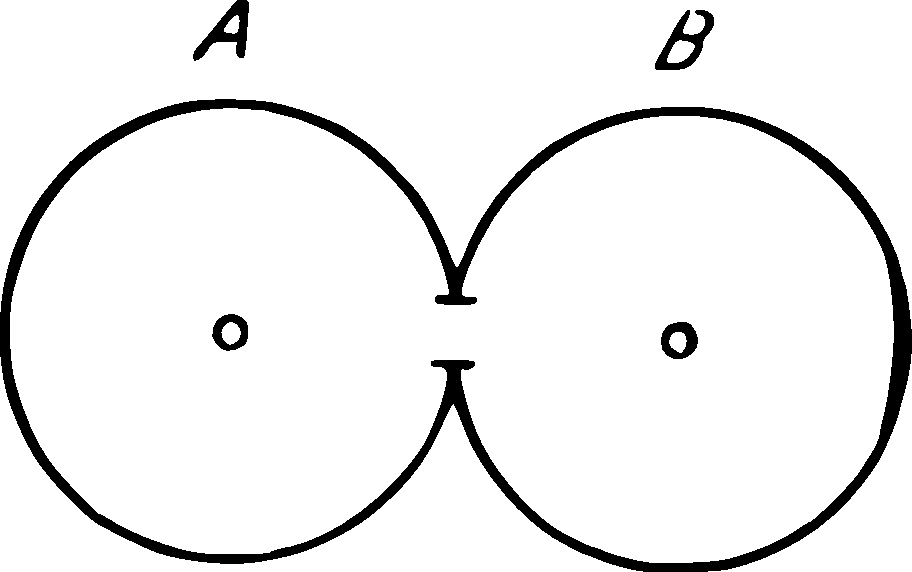
\includegraphics[width=0.8\textwidth]{figs/ch-36/fig-36-01.pdf}
\sidecaption{Heat exchange between two adiabatically closed systems.\zhcap{两个绝热封闭系统之间的热交换。}\label{fig-36-01}}
\end{marginfigure}

It follows from the second law of thermodynamics \ssect{11.3.2} that radiative equilibrium is independent of the material of the bodies that make up the closed thermodynamically equilibrium system. The volume density of the energy of radiation equilibrium and its frequency distribution are universal functions of the temperature. As a matter of fact, if this were not so, it would be possible to take two adiabatically closed systems $A$ and $B$ (\figr{fig-36-01}), at the same temperature $T_{A} = T_{B} = T$,
and accomplish radiative heat exchange between them by making
a small hole in the heatproof wall separating them. If the
volume density of energy $E_{A}^{d}$ of system $A$ is greater than that
$E_{B}^{d}$ of system $B$, i.e. $E_{A}^{d}> E_{B}^{d}$, then, owing to heat exchange between the systems, the radiant energy in system $A$ and its temperature should decrease and the radiant energy in system $B$ and its temperature should increase until the values of the volume energy densities in systems $A$ and $B$ become equal: $E_{A}^{d'} = E_{B}^{d'}$. But, in this case, $T'_{B} > T'_{A}$ so that the process being
considered contradicts the second statement of the second law of thermodynamics \ssect{11.3.2}. Consequently, $E_{A}^{d}$ cannot be greater than $E_{B}^{d}$. In exactly the same way, $E_{B}^{d}$ cannot be greater than $E_{A}^{d}$, i.e. $E_{A}^{d} = E_{B}^{d} = E^{d} (T)$ is a universal function of
the temperature.
\zhpar{由热力学第二定律（见\ssect{11.3.2}）可知，辐射平衡与组成热力学平衡封闭系统的物体的材料无关。辐射平衡的体积能量密度及其频率分布是温度的普适函数。事实上，若非如此，则可取两个温度相同（$T_{A} = T_{B} = T$）的绝热封闭系统 $A$ 和 $B$（见\figr{fig-36-01}），在隔开它们的绝热壁上开一个小孔，使两者之间发生辐射换热。若系统 $A$ 的体积能量密度 $E_{A}^{d}$ 大于系统 $B$ 的 $E_{B}^{d}$，即 $E_{A}^{d}> E_{B}^{d}$，那么由于两系统之间的热交换，系统 $A$ 中的辐射能及其温度将减小，系统 $B$ 中的辐射能及其温度将增大，直至两者的体积能量密度相等，即 $E_{A}^{d'} = E_{B}^{d'}$。但在这种情况下，$T'_{B} > T'_{A}$，所考虑的过程与热力学第二定律的第二种表述（见\ssect{11.3.2}）相矛盾。因此，$E_{A}^{d}$ 不可能大于 $E_{B}^{d}$。同理，$E_{B}^{d}$ 也不可能大于 $E_{A}^{d}$，即 $E_{A}^{d} = E_{B}^{d} = E^{d} (T)$ 是温度的普适函数。}

\subsection{}\label{36.1.3} Serving as the spectral characteristic of radiative equilibrium is the \redem{spectral density of the volume energy denstiy of this radiation}. Thus
\zhpar{辐射平衡的光谱特征量是该辐射的\redem{体积能量密度的谱密度}。于是有}
\begin{equation*}%
\rho (\nu,\, T) = \dv{E^{d}}{\nu},
\end{equation*}
where $\dd E^{d}$ is the energy of radiative equilibrium with frequencies from $\nu$ to $\nu + \dd \nu$ enclosed within unit volume of the radiation field. The volume energy density of this field is
\zhpar{式中 $\dd E^{d}$ 是辐射场单位体积内频率在 $\nu$ 至 $\nu + \dd \nu$ 之间的辐射平衡能量。该辐射场的体积能量密度为}
\begin{equation*}%
E^{d} = \int_{0}^{\infty} \rho (\nu,\, T) \dd \nu.
\end{equation*}
Radiation equilibrium is \redem{isotropic}, i.e. it is not polarized and all directions of its propagation are equally probable. The energy $\dd E$ of radiation equilibrium in vacuum at frequencies from $\nu$ to $\nu + \dd \nu$ incident in unit time on unit area of the surface of each of the bodies of a thermodynamically equilibrium system is equal to
\zhpar{辐射平衡是\redem{各向同性}的，即它不具有偏振，其各传播方向都是等概率的。在真空中，单位时间内以频率从 $\nu$ 到 $\nu + \dd \nu$ 投射到热力学平衡系统中各物体表面单位面积上的辐射平衡能量 $\dd E$ 等于}
\begin{equation*}%
\dd E = \frac{c}{4} \rho (\nu,\, T) \dd \nu.
\end{equation*}
where $c$ is the velocity of light in free space (or in a vacuum).
\zhpar{式中 $c$ 为自由空间（或真空）中的光速。}

\subsection{}\label{36.1.4} The \redem{radiant exitance}\sidenote{Formerly called the radiant emittance.} \redem{(total emissive power)} of a body is the physical quantity $M_{c}$, numerically equal to the energy of
electromagnetic waves of all possible frequencies (or wavelengths) from 0 to $\infty$\sidenote{It is practically sufficient to be restricted to the range of frequencies and wavelengths of optical radiation \ssect{31.4.3}.} radiated in unit time from unit area of a body's surface.
\zhpar{物体的\redem{辐射出射度}（\redem{总发射本领}）是这样一个物理量 $M_{c}$，其数值等于物体表面单位面积在单位时间内辐射出的、所有可能频率（或波长，从 0 到 $\infty$）的电磁波的能量。}
\zhpar{注：旧称辐射发射度（radiant emittance）。}
\zhpar{注：实际上只需考虑光辐射的频率与波长范围即可（见\ssect{31.4.3}）。}



The \redem{emissive power (spectral density of radiant exitance)} of a body is the physical quantity numerically equal to the ratio of the energy $\dd E$ radiated in unit time from unit area of the surface of the body by electromagnetic waves in a narrow range of frequencies from $\nu$ to $\nu + \dd \nu$ (or wavelengths in vacuum from $\lambda$ to $\lambda + \dd \lambda$), to the width of this range:
\zhpar{物体的\redem{发射本领}（\redem{辐射出射度的谱密度}）是这样一个物理量，其数值等于物体表面单位面积在单位时间内、以电磁波形式辐射出的、频率在 $\nu$ 至 $\nu + \dd \nu$（或真空中波长在 $\lambda$ 至 $\lambda + \dd \lambda$）的窄范围内的能量 $\dd E$，与该范围宽度之比：}
\begin{align*}%
r_{\nu} & = \dv{E}{\nu} \qor \\
r_{\lambda} & = \dv{E}{\lambda} = \frac{c}{\lambda^{2}} r_{\nu},
\end{align*}
where $c$ is the velocity of light in vacuum. The values of $r_{\nu}$ (or $r_{\lambda}$) depend upon the frequency (or wavelength), temperature, chemical composition of the body and the condition of its surface.
\zhpar{式中 $c$ 为真空中的光速。$r_{\nu}$（或 $r_{\lambda}$）的值取决于频率（或波长）、物体的温度、化学成分以及表面状况。}

The radiant exitance of a body is related to $r_{\nu}$ and $r_{\lambda}$ by the equations
\zhpar{物体的辐射出射度与 $r_{\nu}$ 和 $r_{\lambda}$ 之间的关系由下列各式给出：}
\begin{equation*}%
M_{e} = \int_{0}^{\infty} r_{\nu} \dd \nu = \int_{0}^{\infty} r_{\lambda} \dd \lambda .
\end{equation*}

\subsection{}\label{36.1.5} The \redem{absorptance (monochromatic absorption coefficient) of a body} is the dimensionless quantity av which indicates what fraction of the energy of electromagnetic waves of frequencies from $\nu$ to $\nu + \dd \nu$, incident on the surface of the body, is absorbed by it. Thus
\zhpar{物体的\redem{吸收本领}（\redem{单色吸收系数}）是一个无量纲量，表示投射到物体表面的、频率从 $\nu$ 到 $\nu + \dd \nu$ 的电磁波能量中，被物体吸收的份额。于是有}
\begin{equation*}%
\alpha_{\nu} = \dv{E_{abs}}{E_{inc}} \leqslant 1. 
\end{equation*}
The value of $\alpha_{\nu}$ depends upon the frequency, temperature, chemical composition of the body and the condition of its surface.
\zhpar{$\alpha_{\nu}$ 的值取决于频率、温度、物体的化学成分以及表面状况。}

\begin{marginfigure}%[-3cm] 
\centering
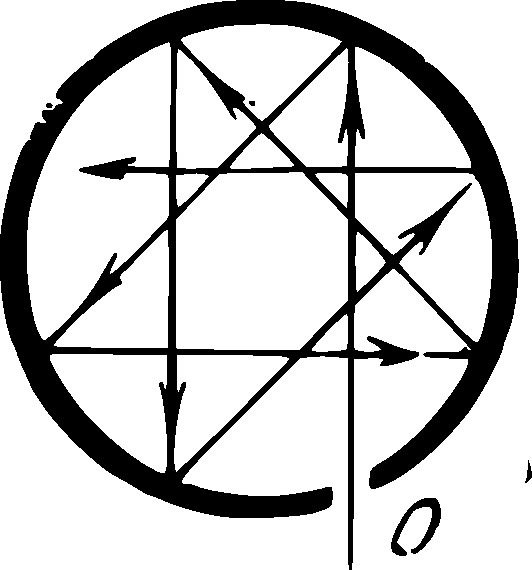
\includegraphics[width=0.5\textwidth]{figs/ch-36/fig-36-02.pdf}
\sidecaption{A blackbody realization in practice.\zhcap{实际中黑体的一种近似实现。}\label{fig-36-02}}
\end{marginfigure}

A \redem{blackbody} (denoted by a superscript asterisk) is one that completely absorbs all incident radiation, regardless of its direction, spectral composition and polarization, without reflecting or transmitting any: $\alpha_{\nu}^{*} \equiv 1$. Though a blackbody is a theoretical ideal, it can be nearly realized in practice by an almost complete enclosure with a small opening (\figr{fig-36-02}). Light entering the enclosure through hole $O$ undergoes repeated reflection from the walls. At this the energy of the incident light is practically completely absorbed by the walls of the enclosure regardless
of the material of which they are made. The emissive power of
a blackbody is denoted in the following by $r_{\nu}^{*}$ (or $r_{\lambda}^{*}$) and its radiant exitance by $M_{e}^{*}$.
\zhpar{\redem{黑体}（以上标星号表示）是能够完全吸收各方向、各光谱成分及各种偏振的入射辐射，既不反射也不透射任何辐射的物体：$\alpha_{\nu}^{*} \equiv 1$。黑体虽是理想化的模型，但在实践中可以用一个带小孔的几乎封闭的空腔近似实现（见\figr{fig-36-02}）。光线经小孔 $O$ 射入后，在腔壁上经历多次反射。在此过程中，入射光的能量几乎被腔壁完全吸收，而与腔壁所用的材料无关。下文中，黑体的发射本领记为 $r_{\nu}^{*}$（或 $r_{\lambda}^{*}$），其辐射出射度记为 $M_{e}^{*}$。}



A \redem{greybody} is one whose absorptance is less than unity and is independent of the frequency (or wavelength) of the light, the directions of its propagation and polarization:
\zhpar{\redem{灰体}是吸收本领小于 1、且与光的频率（或波长）、传播方向以及偏振均无关的物体：}
\begin{equation*}%
\pdv{\alpha_{\nu}^{gr}}{\nu} \equiv 0 \qand \alpha^{gr}_{\nu}  = \alpha^{gr}.
\end{equation*}

\subsection{}\label{36.1.6} According to the \redem{principle of detailed balance} any microscopic process in an equilibrium system should proceed at the same rate as the reverse process. This principle of statistical physics enables a relation to be found between the emissive power $r_{\nu}$ and the absorptance $\alpha_{\nu}$ of any opaque body. Assume that the body is part of a thermodynamically equilibrium system at the temperature $T$. The energy radiated per unit time from unit area of the surface of the body being considered in
the frequency range from $\nu$ to $\nu + \dd \nu$ is
$\dd E_{rad} = r_{nu}\dd \nu$. During the same time, the same portion of the surface of the body absorbs a part of the energy of the radiation equilibrium \ssect{36.1.3} incident on this'surface. It is equal to $\dd E_{abs} = \alpha_{\nu} (c/4) \rho (\nu,\, T) \dd \nu$. Since, according to the principle of detailed balance, $\dd E_{rad} = \dd E_{abs}$,
\zhpar{根据\redem{细致平衡原理}，平衡系统中的任何微观过程都以与其逆过程相同的速率进行。这一统计物理原理使我们能够找到任意不透明物体的发射本领 $r_{\nu}$ 与吸收本领 $\alpha_{\nu}$ 之间的关系。设该物体是温度为 $T$ 的热力学平衡系统的一部分。在单位时间内，该物体表面单位面积在频率从 $\nu$ 到 $\nu + \dd \nu$ 范围内辐射的能量为 $\dd E_{rad} = r_{nu}\dd \nu$。同一时间内，该表面的同一部分还吸收了投射到其上的辐射平衡能量（见\ssect{36.1.3}）的一部分，其值为 $\dd E_{abs} = \alpha_{\nu} (c/4) \rho (\nu,\, T) \dd \nu$。由于根据细致平衡原理有 $\dd E_{rad} = \dd E_{abs}$，故有：}
\begin{equation*}%
\frac{r_{\nu}}{\alpha_{\nu}} = r_{\nu}^{*} = \frac{c}{4} =\rho (\nu, \, T).
\end{equation*}
This equation expresses \redem{Kirchhoff's law} (for radiation), which states that the ratio of the emissive power of a body to its absorptance does not depend upon the nature of the body and is equal to the emissive power $r_{\nu}^{*}$ of a blackbody at the same temperature and frequency values.
\zhpar{上式即为（辐射的）\redem{基尔霍夫定律}，它表明：物体的发射本领与其吸收本领之比不依赖于物体的性质，并且等于在相同温度和频率下黑体的发射本领 $r_{\nu}^{*}$。}

The dependence of $r_{\nu}^{*}$ on $\nu$ and $T$ is called \redem{Kirchhoff's function}:
\zhpar{$r_{\nu}^{*}$ 对 $\nu$ 和 $T$ 的依赖关系称为\redem{基尔霍夫函数}：}
\begin{equation*}%
r_{\nu}^{*} = f(\nu, \, T) = \frac{c}{4} =\rho (\nu, \, T).
\end{equation*}

\subsection{}\label{36.1.7} It follows from Kirchhoff's law that the radiant exitance \ssect{36.1.4} of a body is equal to
\zhpar{由基尔霍夫定律可知，物体的辐射出射度（见\ssect{36.1.4}）等于}
\begin{equation*}%
M_{e} = \int_{0}^{\infty} \alpha_{\nu} r_{\nu}^{*} \dd \nu.
\end{equation*}
In particular, the radiant exitance of a greybody is
\begin{equation*}%
M_{e}^{gr} = \alpha^{gr} M_{e}^{*}, \text{ where } M_{e}^{*} = \int_{0}^{\infty}  r_{\nu}^{*} \dd \nu,
\end{equation*}
is the radiant exitance of a blackbody at the same temperature. For a nongrey body
\zhpar{此处 $M_{e}^{*}$ 为同一温度下黑体的辐射出射度。对于非灰体，有}
\begin{equation*}%
M_{e} = \beta M_{e}^{*},
\end{equation*}
where $\beta$ is the \redem{total degree of blackness of the body}. It depends on the material of the body, the condition of its surface and the temperature. For all bodies except a blackbody, $\beta < 1$.
\zhpar{式中 $\beta$ 为物体的\redem{总黑度}。它取决于物体的材料、表面状况以及温度。除黑体外，所有物体的 $\beta < 1$。}

\subsection{}\label{36.1.8} Radiation equilibrium at the temperature $T$ is identical to thermal radiation of a blackbody at the same temperature. Therefore, it is often called \redem{blackbody radiation}. The relation between the radiant exitance of a blackbody and the volume density
of the energy of blackbody radiation is of the form
\zhpar{温度为 $T$ 的辐射平衡与同温度下黑体的热辐射完全相同，因此它常被称为\redem{黑体辐射}。黑体的辐射出射度与黑体辐射的体积能量密度之间的关系具有如下形式}
\begin{equation*}%
M_{e}^{*} = \frac{c}{4} E^{d} = \frac{c}{4} \int_{0}^{\infty}  \rho (\nu, \, T)  \dd \nu.
\end{equation*}

\section{Stefan-Boltzmann and Wien Laws}
\label{sec-36.2} 
\zhtitle{斯特藩-玻尔兹曼定律与维恩定律}



\subsection{}\label{36.2.1} The \redem{Stefan-Boltzmann law} states that the radiant exitance of a blackbody is proportional to the fourth power of its absolute temperature. Thus
\zhpar{\redem{斯特藩-玻尔兹曼定律}指出：黑体的辐射出射度与其绝对温度的四次方成正比。即}
\begin{equation*}%
M_{e}^{*} = \sigma T^{4},
\end{equation*}
where $\sigma = \SI{5.67d-8}{\watt\per\meter\squared\kelvin\tothe{4}}$ is the \redem{Stefan-Boltzmann constant}. This law can be derived theoretically by considering the radiative equilibrium in an enclosed cavity by thermodynamic methods.
\zhpar{式中 $\sigma$ 为\redem{斯特藩-玻尔兹曼常量}。该定律可以通过热力学方法考察封闭空腔内的辐射平衡，从理论上导出。}


\begin{marginfigure}[0cm] 
\centering
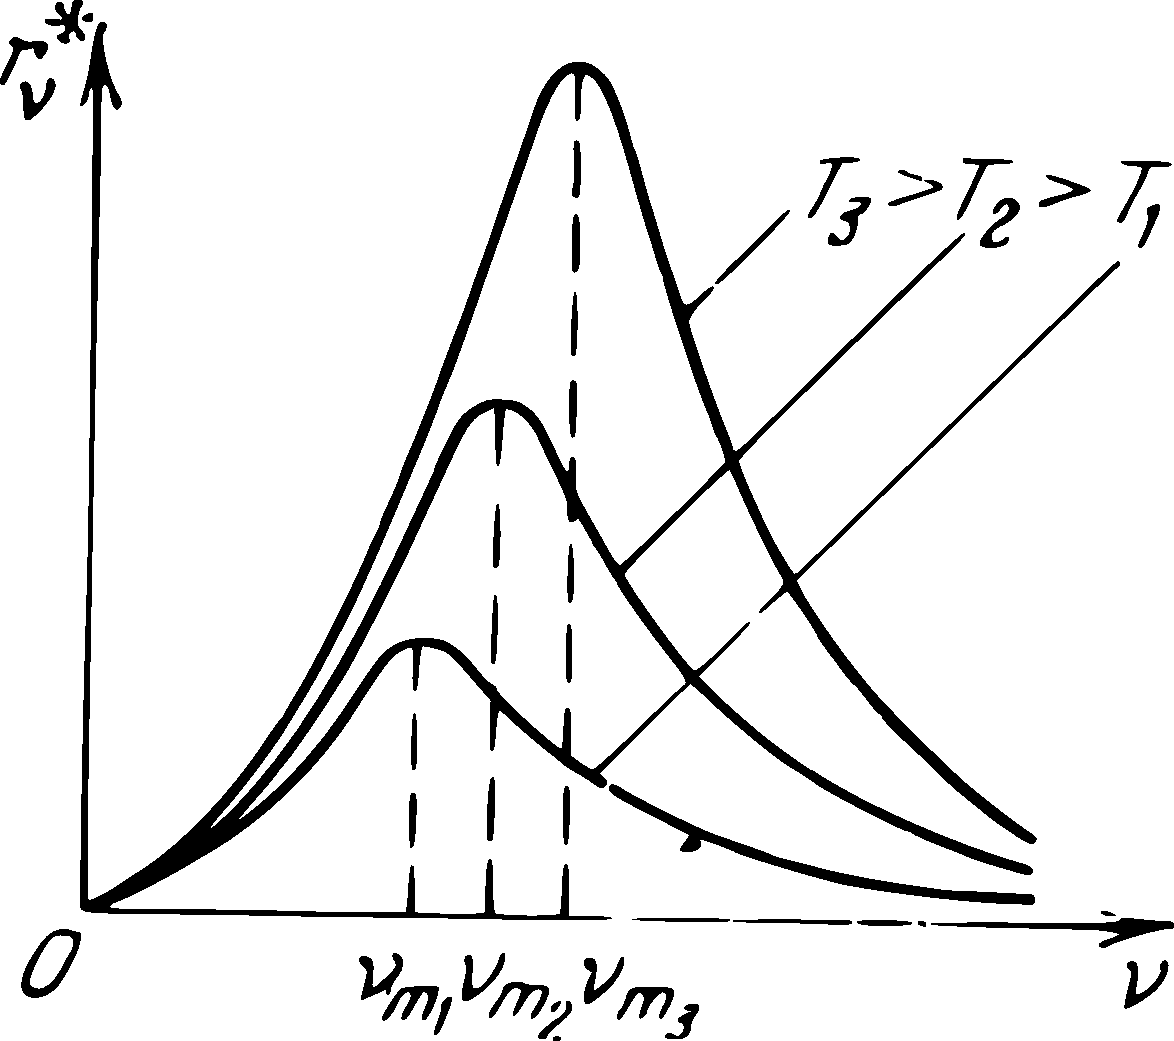
\includegraphics[width=\textwidth]{figs/ch-36/fig-36-03.pdf}
\sidecaption{ The dependence of the emissive power $r_{\nu}^{*}$ of a blackbody on the frequency $\nu$. \zhcap{黑体的发射本领 $r_{\nu}^{*}$ 随频率 $\nu$ 的变化。}\label{fig-36-03}}
\end{marginfigure}

\subsection{}\label{36.2.2} The dependence of the emissive power $r_{\nu}^{*}$ of a blackbody on the frequency $\nu$ for several constant values of the temperature is shown in \figr{fig-36-03}. In the region of low frequencies, $r_{\nu}^{*}\propto \nu^{2}T$, whereas for the region of high frequencies (the right-hand branch of the curves far away from the maxima) $r_{\nu}^{*}\propto \nu^{3} \exp [-a_{1\nu/T}]$, where $a_{1}$ is a constant factor.
\zhpar{黑体的发射本领 $r_{\nu}^{*}$ 随频率 $\nu$ 的变化关系，在温度取若干固定值时如\figr{fig-36-03}所示。在低频区，$r_{\nu}^{*}\propto \nu^{2}T$；而在高频区（曲线远离极大值的右侧分支），$r_{\nu}^{*}\propto \nu^{3} \exp [-a_{1\nu/T}]$，其中 $a_{1}$ 为常数因子。}

The radiant energy of a blackbody is nonuniformly distributed
in its spectrum. A blackbody displays almost no radiation in the regions of very high and very low frequencies. As the temperature is raised, the maximum of $r_{\nu}^{*}$ is shifted toward thehigher frequencies in accordance with the law: $\nu_{m} = b_{1}T$, where $\nu_{m}$ is the frequency corresponding to maximum $r_{\nu}^{*}$ at the temperature $T$, and $b_{1}$ is a constant factor.
\zhpar{黑体的辐射能在其光谱中的分布是不均匀的。在频率很高和很低的区域，黑体几乎不辐射。随着温度升高，$r_{\nu}^{*}$ 的极大值向高频方向移动，其规律为 $\nu_{m} = b_{1}T$，其中 $\nu_{m}$ 是温度为 $T$ 时使 $r_{\nu}^{*}$ 取极大值的频率，$b_{1}$ 为常数因子。}

\begin{marginfigure}[-1cm] 
\centering
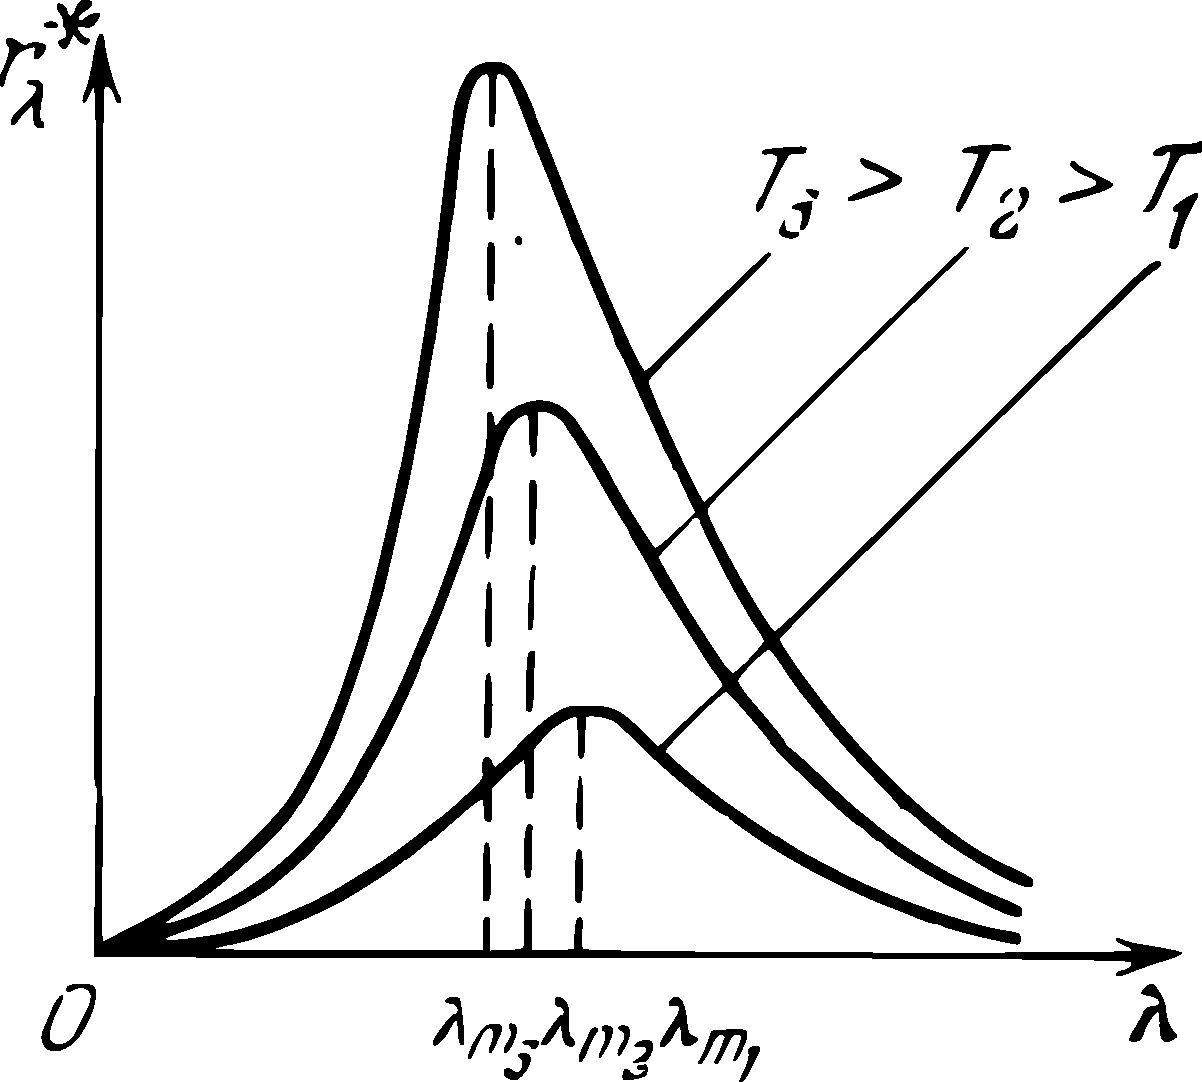
\includegraphics[width=\textwidth]{figs/ch-36/fig-36-04.pdf}
\sidecaption{ The dependence of the emissive power $r_{\nu}^{*}$ of a blackbody on the wavelength $\lambda$. \zhcap{黑体的发射本领 $r_{\nu}^{*}$ 随波长 $\lambda$ 的变化。}\label{fig-36-04}}
\end{marginfigure}


The dependence of the emissive power of a blackbody $r_{\lambda}^{*}= c r_{\nu}^{*}/\lambda^{2}$ \ssect{36.1.4} on the wavelength $\lambda$ is shown in \figr{fig-36-04}.
\zhpar{黑体的发射本领 $r_{\lambda}^{*}= c r_{\nu}^{*}/\lambda^{2}$（见\ssect{36.1.4}）随波长 $\lambda$ 的变化关系如\figr{fig-36-04}所示。}

As the temperature of the blackbody is raised, the maximum of
rj is shifted toward the shorter wavelengths in accordance with the \redem{Wien displacement law}:
\zhpar{随着黑体温度升高，其发射本领的极大值向短波方向移动，遵循\redem{维恩位移定律}：}
\begin{equation*}%
\lambda_{m} = \frac{b}{T},
\end{equation*}
where $b = \SI{2.9d-3}{\meter\kelvin}$ is the \redem{Wien constant}.
\zhpar{式中 $b$ 为\redem{维恩常量}。}

\subsection{}\label{36.2.3} All attempts that were made failed to theoretically sub­ stantiate the experimentally found form of Kirchhoff's function, $r_{\nu}^{*} = f (\nu,\, T)$, shown in \figr{fig-36-03}, within the framework of classical physics. Using thermodynamic methods, the \redem{Wien formula} was found:
\zhpar{在经典物理学的框架内，所有试图从理论上论证实验所得基尔霍夫函数形式 $r_{\nu}^{*} = f (\nu,\, T)$（见\figr{fig-36-03}）的努力都未能成功。利用热力学方法，得到了\redem{维恩公式}：}
\begin{equation*}%
r_{\nu}^{*} = \nu^{3} \varphi \left( \frac{\nu}{T} \right),
\end{equation*}
where $\varphi (\nu/T)$ is an unknown function of $\nu/T$.
\zhpar{式中 $\varphi (\nu/T)$ 是 $\nu/T$ 的未知函数。}

Rayleigh and Jeans applied the laws of electrodynamics and
equipartition of energy in an equilibrium system \ssect{10.6.4} to obtain the \redem{Rayleigh-Jeans law}:
\zhpar{瑞利和金斯应用电动力学定律以及平衡系统中的能量均分原理（见\ssect{10.6.4}），得到了\redem{瑞利-金斯定律}：}
\begin{equation*}%
r_{\nu}^{*} = \frac{2 \pi \nu^{2}}{c^{2}} kT,
\end{equation*}
where $k$ is Boltzmann's constant \ssect{8.4.5}.
\zhpar{式中 $k$ 为玻尔兹曼常量（见\ssect{8.4.5}）。}

The Rayleigh-Jeans law agreed with experimental data only
in the region of low frequencies. Moreover, it leads to the absurd conclusion that at any temperature the radiant exitance
$M_{e}^{*}$ of a blackbody and the volume density of energy $E^{d}$ of radiation equilibrium are inhnitely large. This conclusion, arrived at by classical physics in the problem of explaining the spectral distribution of radiation equilibrium, has been aptly named the ``ultraviolet catastrophe''.
\zhpar{瑞利-金斯定律仅在低频区域与实验数据相符。此外，它还导出了一个荒谬的结论：在任何温度下，黑体的辐射出射度 $M_{e}^{*}$ 和辐射平衡的体积能量密度 $E^{d}$ 都将是无穷大。经典物理学在解释辐射平衡的光谱分布问题时得出的这一结论，被恰当地称为“\redem{紫外灾难}”。}

\section{Planck's Formula}
\label{sec-36.3} 
\zhtitle{普朗克公式}


\subsection{}\label{36.3.1} The volume density of energy of radiation equilibrium (blackbody radiation) in a closed cavity, as well as the energy distribution of this radiation in frequency are independent of the material of the cavity walls and are fully determined by the temperature. Therefore, an infinite system of harmonic oscillators with all possible natural frequencies can be taken as a theoretical model of a blackbody. Each of such oscillat ors corresponds to a monochromatic component of blackbody radiation. Let
$\expval{E_{\nu}}$ be the average energy of an oscillator with the natural frequency $\nu$. Then, according to calculations, the radiant exitance of a blackbody is
\zhpar{设 $\expval{E_{\nu}}$ 为固有频率为 $\nu$ 的振子的平均能量。于是，经计算，黑体的辐射出射度为}
\begin{equation*}%
r_{\nu}^{*} = \frac{2 \pi \nu^{2}}{c^{2}}\expval{E_{\nu}},
\end{equation*}
If $kT$ is taken for $\expval{E_{\nu}}$, as follows from the classical law of the equipartition of energy \ssect{10.6.4}\sidenote{One oscillatory degree of freedom of an oscillator accounts for twice as much energy, on an average, as one degree of translational or rotary motion, because the oscillator has not only kinetic, but potential energy as well. On an average, this potential energy is equal to the kinetic energy.}, then the preceding expression
for $r_{\nu}^{*} $ coincides with the Rayleigh-Jeans law \ssect{36.2.3}.
\zhpar{若取 $kT$ 作为 $\expval{E_{\nu}}$（由经典的能量均分定律得出，见\ssect{10.6.4}），则上式中的 $r_{\nu}^{*}$ 与瑞利-金斯定律（见\ssect{36.2.3}）相吻合。}
\zhpar{注：振子的一个振动自由度平均所具有的能量，是一个平动或转动自由度能量的两倍，因为振子不仅有动能，还有势能。平均而言，这一势能等于动能。}

\subsection{}\label{36.3.2} Planck was able to find the correct expression for the average energy  $\expval{E_{\nu}}$ of an oscillator and for the Kirchhoff function by introducing the \redem{quantum hypothesis}, which was entirely alien to classical physics. It is assumed in classical physics that the energy of any system can vary in a \redem{continuous manner},
i.e. that it can take any arbitrarily close consecutive values.
\zhpar{普朗克引入了完全不属于经典物理学的\redem{量子假设}，从而找到了振子平均能量 $\expval{E_{\nu}}$ 以及基尔霍夫函数的正确表达式。经典物理学认为，任何体系的能量都可以以\redem{连续的方式}变化，即能量可以取任意相互接近的相继数值。}

According to Planck's quantum hypothesis, the energy
$\expval{E_{\nu}}$ of an oscillator can have only definite \redem{discrete (quantized)} values, equal to a whole number of elementary portions, called \redem{energy quanta} $E_{\nu \, 0}$. Thus
\zhpar{根据普朗克量子假设，振子的能量 $\expval{E_{\nu}}$ 只能取某些确定的\redem{离散（量子化）}数值，它们等于基本能量份额——\redem{能量子} $E_{\nu \, 0}$——的整数倍。即}
\begin{equation*}%
 E_{\nu} = n E_{\nu \, 0}, \text{ where } n = 0, \,1, \,2, \ldots{}
\end{equation*}
If it is assumed that the oscillator distribution in possible discrete energy states is described by the Boltzmann distribution law \ssect{10.4.2}, the probability pn of finding the oscillator in a state with the energy $nE_{nu\, 0}$ at the temperature $T$ is equal to
\zhpar{若假定振子在可能的离散能量状态中的分布服从\redem{玻尔兹曼分布律}（见\ssect{10.4.2}），则在温度 $T$ 下，振子处于能量为 $nE_{nu\, 0}$ 的状态的概率 $p_{n}$ 等于}
\begin{equation*}%
p_{n} = C \exp \left[ \frac{-nE_{\nu\, 0}}{kT} \right].
\end{equation*}
Here $k$ is the Boltzmann constant \ssect{8.4.5} and $C$ is a constant factor determined from the normalization condition:
\zhpar{式中 $k$ 为玻尔兹曼常量（见\ssect{8.4.5}），$C$ 为由归一化条件确定的常数因子：}
\begin{equation*}%
\sum_{n =0}^{\infty} p_{n} = 1, \text{ i.e. } C = \frac{1}{\sum_{n =0}^{\infty} \exp \left[ \dfrac{-nE_{\nu\, 0}}{kT} \right]}.
\end{equation*}
The average value of the oscillator energy is
\zhpar{振子能量的平均值为}
\begin{equation*}%
\expval{E_{\nu}} = \sum_{n =0}^{\infty} p_{n} n E_{\nu\, 0} = E_{\nu\, 0} \frac{\sum_{n =0}^{\infty}n \exp \left[ \dfrac{-nE_{\nu\, 0}}{kT} \right]}{\sum_{n =0}^{\infty} \exp \left[ \dfrac{-nE_{\nu\, 0}}{kT} \right]},
\end{equation*}
from which
\zhpar{由此得到}
\begin{align*}%
\expval{E_{\nu}} & = -  E_{\nu\, 0}  \frac{\dv{\xi} \sum_{n =0}^{\infty} n \exp (-n \xi)}{\sum_{n =0}^{\infty} \exp (- n \xi)}\\
& = -  E_{\nu\, 0}\dv{\xi} \ln \sum_{n =0}^{\infty} \exp (- n \xi),
\end{align*}
where $\xi = E_{\nu \,0}/kT$. Since
\zhpar{式中 $\xi = E_{\nu \,0}/kT$。由于}
\begin{align*}%
\sum_{n =0}^{\infty} \exp (- n \xi) & = \frac{1}{1 - \exp(-\xi)} \qand \\
-\ln \sum_{n =0}^{\infty} \exp (- n \xi) & = \ln (1 - \exp(-\xi)), \text{ then} \\
\expval{E_{\nu}} & =   \frac{E_{\nu\, 0}}{\exp \left[ \dfrac{E_{\nu\, 0}}{kT}\right] -1} \qand \\
r_{\nu}^{*} & =  \frac{2\pi \nu^{2}}{c^{2}} \frac{E_{\nu\, 0}}{\exp \left[ \dfrac{E_{\nu\, 0}}{kT}\right] -1}.
\end{align*}
Comparing this expression for $r_{\nu}^{*}$ with the Wien formula \ssect{36.2.3}, it follows that a \redem{quantum of energy} is equal to
\zhpar{将此 $r_{\nu}^{*}$ 的表达式与维恩公式（见\ssect{36.2.3}）比较，可知\redem{能量子}为}
\begin{equation*}%
E_{\nu\, 0} = h\nu,
\end{equation*}
where $h$ is a universal constant, called \redem{Planck's constant} (Appendix~II).
\zhpar{式中 $h$ 为普适常量，称为\redem{普朗克常量}（见附录 II）。}

\redem{Planck's radiation formula} for the emissive power $r_{\nu}^{*}$ of a blackbody is
\zhpar{黑体发射本领 $r_{\nu}^{*}$ 的\redem{普朗克辐射公式}为}
\begin{equation*}%
r_{\nu}^{*} =  \frac{2\pi \nu^{2}}{c^{2}} \frac{h \nu}{\exp \left[ \dfrac{h \nu}{kT}\right] -1}.
\end{equation*}
Accordingly, the \redem{spectral density of radiation equilibrium} \ssect{36.1.3} is equal to
\zhpar{相应地，\redem{辐射平衡的谱密度}（见\ssect{36.1.3}）等于}
\begin{equation*}%
\rho (\nu, \, T)  =  \frac{8\pi \nu^{2}}{c^{3}} \frac{h \nu}{\exp \left[ \dfrac{h \nu}{kT}\right] -1}.
\end{equation*}

\subsection{}\label{36.3.3} At low frequencies $(h \nu \ll kT)$, $\exp [h\nu/kT - 1] \approx h\nu/kT$ and the Planck radiation formula coincides with the Rayleigh-Jeans law \ssect{36.2.3}.
\zhpar{在低频区（$h \nu \ll kT$），$\exp [h\nu/kT - 1] \approx h\nu/kT$，普朗克辐射公式与瑞利-金斯定律（见\ssect{36.2.3}）相吻合。}

Following from Planck's radiation formula is the Stefan-Boltzmann law \ssect{36.2.1}:
\zhpar{由普朗克辐射公式可以导出斯特藩-玻尔兹曼定律（见\ssect{36.2.1}）：}
\begin{align*}%
M_{e}^{*} & = \frac{2 \pi h}{c^{2}} \int_{0}^{\infty} \frac{\nu^{3} \dd \nu}{\exp \left[ \dfrac{h \nu}{kT}\right] -1}\\
& = \frac{2 \pi k^{4}T^{4}}{c^{2}h^{3}} \int_{0}^{\infty} \frac{\eta^{3} \dd \eta}{\exp \eta -1} = \frac{2 \pi^{5} k^{4}}{15 c^{2}h^{3}} T^{4}.
\end{align*}
The Planck constant is related to the Stefan-Boltzmann constant $\sigma$ \ssect{36.2.1} as follows:
\zhpar{普朗克常量与斯特藩-玻尔兹曼常量 $\sigma$（见\ssect{36.2.1}）之间的关系如下：}
\begin{equation*}%
h = \sqrt[3]{\frac{2 \pi^{5}k^{4}}{15c^{2} \sigma}} = \SI{6.62d-34}{\joule\second}.
\end{equation*}

\subsection{}\label{36.3.4} The Planck formula for the emissive power $r_{\lambda}^{*}$ of a black-body is
\zhpar{黑体发射本领 $r_{\lambda}^{*}$ 的普朗克公式为}
\begin{equation*}%
r_{\lambda}^{*} = \frac{2 \pi c^{2}h}{\lambda^{5}} \frac{1}{\exp \left[ \dfrac{hc}{\lambda k T}\right] - 1}.
\end{equation*}
The wavelength $\lambda_{m}$ corresponding to maximum $r_{\lambda}^{*}$ is determined from the transcendental equation
\zhpar{使 $r_{\lambda}^{*}$ 取极大值的波长 $\lambda_{m}$ 由下列超越方程确定：}
\begin{equation*}%
xe^{x} - 5e^{x} + 5 = 0, \text{ where } x = hc/\lambda_{m}kT.
\end{equation*}
The root of this equation $x = 4.965$, and $\lambda_{m}$ satisfies the Wien displacement law \ssect{36.2.2}:
\zhpar{该方程的根为 $x = 4.965$，且 $\lambda_{m}$ 满足维恩位移定律（见\ssect{36.2.2}）：}
\begin{equation*}%
\lambda_{m} T = b, \text{ where } b = \frac{hc}{\SI{4.965}{\kelvin}} = \SI{2.9d-3}{\meter\kelvin}.
\end{equation*}





\section{Optical Pyrometry}
\label{sec-36.4} 
\zhtitle{光学测温法}



\subsection{}\label{36.4.1} \redem{Optical pyrometry} is the name given to miscellaneous techniques for measuring high temperatures based on the laws of thermal radiation. The instruments used for this purpose are called \redem{pyrometers}.
\zhpar{\redem{光学测温法}是指基于热辐射定律测量高温的各种技术的统称。用于此目的的仪器称为\redem{高温计}。}

\redem{Radiation pyrometers} record the integrated radiation of the heated body being investigated; optical pyrometers record the radiation of a heated body in one or two narrow portions of the spectrum.
\zhpar{\redem{辐射高温计}记录被研究的加热物体的全部辐射；\redem{光学高温计}则记录加热物体在光谱中一个或两个窄波段内的辐射。}

\subsection{}\label{36.4.2} The \redem{radiant flux} $\Phi_{e}$ is the average power of optical radiation \ssect{31.4.3} during a time considerably greater than a period of oscillation of the electromagnetic field of the light.
\zhpar{\redem{辐射通量} $\Phi_{e}$ 是光辐射（见\ssect{31.4.3}）在远大于光电磁场振动周期的时间内的平均功率。}

The \redem{irradiance} $E_{e}$ (\redem{radiant flux density}) of a surface is the ratio of the flux of incident radiation on this surface to its area. Thus $E_{e} = \dv*{\Phi_{e}}{S}$, where $\dd \Phi_{e}$ is the radiant flux incident on a portion
of the surface of area $\dd S$.
\zhpar{表面的\redem{辐照度} $E_{e}$（\redem{辐射通量密度}）是投射到该表面的辐射通量与其面积之比。即 $E_{e} = \dv*{\Phi_{e}}{S}$，其中 $\dd \Phi_{e}$ 为投射到面积为 $\dd S$ 的表面部分上的辐射通量。}

The \redem{radiant intensity} $I_{e}$ of a radiative body is the radiant flux emitted by the body within a unit solid angle. Thus $I_{e} = \dv*{\Phi_{e}}{\Omega}$, where $\dd \Phi_{e}$ is the radiant flux within the solid angle $\dd \Omega$.
\zhpar{辐射体的\redem{辐射强度} $I_{e}$ 是辐射体在单位立体角内发出的辐射通量。即 $I_{e} = \dv*{\Phi_{e}}{\Omega}$，其中 $\dd \Phi_{e}$ 为立体角 $\dd \Omega$ 内的辐射通量。}

\subsection{}\label{36.4.3} The \redem{radiance} $L_{e}$ of the portion $\dd S$ of a radiative surface in a given direction is the ratio of the radiant intensity $\dd I_{e}$
of area $\dd S$ in the direction being considered to the area of the projection of dS on a plane perpendicular to the direction. Thus
\zhpar{辐射表面上面积元 $\dd S$ 在给定方向上的\redem{辐亮度} $L_{e}$，是该方向上面积 $\dd S$ 的辐射强度 $\dd I_{e}$ 与 $\dd S$ 在垂直于该方向的平面上的投影面积之比。即}
\begin{equation*}%
L_{e} = \frac{\dd I_{e}}{\dd S \cos \varphi}
\end{equation*}
where $\varphi$ is the angle between the specified direction and the normal to the surface of area $\dd S$.
\zhpar{式中 $\varphi$ 为指定方向与面积为 $\dd S$ 的表面法线之间的夹角。}

The \redem{spectral density of the radiance} is the ratio of the radiance $\dd L_{e}$, corresponding to a narrow band of the optical spectrum, to the width of this band. Thus
\zhpar{\redem{辐亮度的谱密度}是对应于光谱中一个窄带的辐亮度 $\dd L_{e}$ 与该波段宽度之比。即}
\begin{equation*}%
b_{\nu} = \dv{L_{e}}{\nu} \qand b_{\lambda} = \dv{L_{e}}{\lambda}.
\end{equation*}

\subsection{}\label{36.4.4} A source of optical radiation is said \redem{to obey Lambert's law}, or \redem{to be a cosine radiator}, if its radiance $L_{e}$, as well as its spectral densities $b_{\nu}$ and $b_{\lambda}$ are the same in all directions, i.e. are independent of angle $\varphi$. A blackbody could be called a cosine radiator.
\zhpar{若光源的辐亮度 $L_{e}$ 及其谱密度 $b_{\nu}$、$b_{\lambda}$ 在所有方向上都相同，即与角度 $\varphi$ 无关，则称该光源服从\redem{朗伯定律}，或称其为\redem{余弦辐射体}。黑体可以称为余弦辐射体。}

The radiance of a cosine radiator and its spectral densities are related to its radiant exitance and its spectral densities \ssect{36.1.4} as follows:
\zhpar{余弦辐射体的辐亮度及其谱密度与其辐射出射度及其谱密度（见\ssect{36.1.4}）之间的关系如下：}
\begin{equation*}%
L_{e} = \frac{M_{e}}{\pi}, \quad b_{\nu} = \dv{r_{\nu}}{\pi} \qand b_{\lambda} = \dv{r_{\lambda}}{\pi}.
\end{equation*}


\subsection{}\label{36.4.5} In optical pyrometry, distinction is made between radiation, brightness and colour temperatures of a body.
\zhpar{在光学测温中，需要区分物体的辐射温度、亮度温度和色温度。}

The \redem{radiation temperature} $T_{r}$ of a body is the temperature of a blackbody at which its radiance $L_{e}^{*}$ is equal to the radiance $L_{e}$ of the given body. If the body being investigated is a cosine radiator, whose total degree of blackness is $\beta$ \ssect{36.1.7}, then,
from the condition that $L_{e} (T) = L_{e}^{*} (T_{r})$, where $T$ is the true temperature of the body, it follows that
\zhpar{物体的\redem{辐射温度} $T_{r}$ 是这样一个黑体的温度，该黑体的辐亮度 $L_{e}^{*}$ 等于被研究物体的辐亮度 $L_{e}$。若被研究物体是余弦辐射体，其总黑度为 $\beta$（见\ssect{36.1.7}），则由条件 $L_{e} (T) = L_{e}^{*} (T_{r})$（式中 $T$ 为物体的真实温度）可得}
\begin{align*}%
\beta M_{e}^{*} (T) & = M_{e}^{*} (T_{r}) \qand \\
T & = \frac{T_{r}}{\sqrt[4]{\beta}} \geqslant T_{r}.
\end{align*}

\subsection{}\label{36.4.6} The \redem{brightness (luminance) temperature} $T_{b}$ of a body is the temperature of a blackbody at which its spectral density $b_{\lambda}^{*}$ of radiance for a definite wavelength $\lambda_{0}$ is equal to the spectral density $b_{\lambda}$ of radiance for the given body for the same wavelength: $b_{\lambda} (\lambda_{0}, T) = b_{\lambda}^{*}(\lambda_{0}, T_{b})$. Usually $\lambda_{0} =   \SI{660}{\nano\meter}$ (red light).
\zhpar{物体的\redem{亮度温度} $T_{b}$ 是这样一个黑体的温度，该黑体对某一确定波长 $\lambda_{0}$ 的辐亮度谱密度 $b_{\lambda}^{*}$，等于被研究物体在同一波长下的辐亮度谱密度 $b_{\lambda}$：$b_{\lambda} (\lambda_{0}, T) = b_{\lambda}^{*}(\lambda_{0}, T_{b})$。通常取 $\lambda_{0} = \SI{660}{\nano\meter}$（红光）。}

For a cosine radiator, whose absorptance \ssect{36.1.5} for light of the wavelength  $\lambda_{0}$ at the temperature $T$ of the body is equal to $\alpha_{\lambda} (\lambda_{0}, T)$, it follows from Kirchholf's law \ssect{36.1.6} and from
Planck's formula \ssect{36.3.4} that
\zhpar{对于余弦辐射体，其温度为 $T$ 时对波长为 $\lambda_{0}$ 的光的吸收本领（见\ssect{36.1.5}）为 $\alpha_{\lambda} (\lambda_{0}, T)$，由基尔霍夫定律（见\ssect{36.1.6}）及普朗克公式（见\ssect{36.3.4}）可知}
\begin{equation*}%
\alpha_{\lambda} (\lambda_{0}, T)\, r_{\lambda}^{*} (\lambda_{0}, T) =  r_{\lambda}^{*} (\lambda_{0}, T_{b}),
\end{equation*}
and
\begin{equation*}%
\alpha_{\lambda} (\lambda_{0}, T)\left[ \exp \left(\frac{a_{2}}{\lambda_{0}T_{b}}\right) - 1 \right] = \exp \left(\frac{a_{2}}{\lambda_{0}T}\right) - 1, 
\end{equation*}
where $a_{2} = hc/k$. Since $a_{\lambda}(\lambda_{0}, T) \leqslant 1$, then $T \geqslant T_{b}$.
\zhpar{式中 $a_{2} = hc/k$。由于 $a_{\lambda}(\lambda_{0}, T) \leqslant 1$，故 $T \geqslant T_{b}$。}

\subsection{}\label{36.4.7} The \redem{colour temperature} $T_{c}$ of a body is the temperature of a blackbody at which the relative distributions of the spectral density of the radiance $b_{\lambda}^{*}$ of the blackbody and that $b_{\lambda}$ of the body being considered are close to one another to the maximum degree in the visible region of the spectrum. Thus
\zhpar{物体的\redem{色温度} $T_{c}$ 是这样一个黑体的温度，该黑体辐亮度谱密度 $b_{\lambda}^{*}$ 的相对分布，与被研究物体辐亮度谱密度 $b_{\lambda}$ 的相对分布，在可见光谱区域内最大限度地相互接近。即}
\begin{equation*}%
\frac{b_{\lambda} (\lambda_{1}, T)}{b_{\lambda} (\lambda_{2}, T)} = \frac{b_{\lambda}^{*} (\lambda_{1}, T_{c})}{b_{\lambda}^{*} (\lambda_{2}, T_{c})} .
\end{equation*}
For a cosine radiator
\zhpar{对于余弦辐射体，有}
\begin{equation*}%
\frac{r_{\lambda} (\lambda_{1}, T)}{r_{\lambda} (\lambda_{2}, T)} = \frac{r_{\lambda}^{*} (\lambda_{1}, T_{c})}{r_{\lambda}^{*} (\lambda_{2}, T_{c})} .
\end{equation*}
As a rule, $\lambda_{1} = \SI{655}{\nano\meter}$ (red light) and $\lambda_{1} = \SI{470}{\nano\meter}$ (green light). The colour temperature of a greybody \ssect{36.1.5} coincides with its true temperature and can be found by Wien's displacement law \ssect{36.2.2}.
\zhpar{通常取 $\lambda_{1} = \SI{655}{\nano\meter}$（红光）和 $\lambda_{1} = \SI{470}{\nano\meter}$（绿光）。灰体（见\ssect{36.1.5}）的色温度与其真实温度一致，可由维恩位移定律（见\ssect{36.2.2}）求得。}



% Local Variables:
% TeX-master: "handbook-physics"
% coding: utf-8
% End:
